% Drawing 138/06-39 -- folder 138, batch 06, archive page 117 (PDF page 118).
% Transcription: un segment à trois sommets ; séparé par un trait courbe, un tripode dans une boucle, marqué $\times$.
% Kind: small maps. Method 2 (schematic redraw from the facsimile). Status: ok.
% Notes: A segment with three vertices; separated by a long curved stroke, a tripod in a loop (the vertex carries the loop and three edges), marked ×. His small crosses beside some maps are kept as × marks. Small planar maps listed by degree (number of edges) in the text; redrawn, not encoded (each would be a map/1 with at most a few edges; the text gives the classification).
% Coordinates: 1 unit = 1 mm = 1/100 of the crop width (bbox in page fractions: [0.55, 0.173, 0.87, 0.229]).
% Redrawn by Claude (claude-opus-5-5), issue #73, 2026-11-07; not checked by a human; not compiled (no TeX in the session).
% Rights: reproduces part of the work -- behind RENDER_TRANSCRIPTS, never published by itself.
\documentclass[tikz,border=3pt]{standalone}
\usepackage{amsmath,amssymb}
\usetikzlibrary{patterns,arrows.meta}
\tikzset{pencil/.style={black!45}, struck/.style={black!35}, mark/.style={circle,draw,inner sep=1.3pt}, pt/.style={circle,fill,inner sep=0.9pt}, opt/.style={circle,draw,fill=white,inner sep=1.1pt}}
\begin{document}
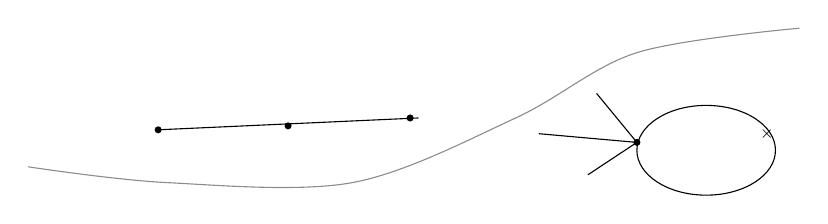
\begin{tikzpicture}[x=1mm,y=1mm,line cap=round,line join=round,font=\scriptsize]
\draw (16.5,-13.9) -- (49.5,-12.4);
\node[pt] at (16.5,-13.9) {};
\node[pt] at (33,-13.4) {};
\node[pt] at (48.5,-12.4) {};
\draw[pencil] plot[smooth, tension=0.55] coordinates {(0,-18.6) (17.5,-20.6) (41.2,-20.6) (61.9,-12.4) (77.3,-4.1) (97.9,-1)};
\draw (86.1,-16.5) ellipse[x radius=8.8, y radius=5.7];
\draw (77.3,-15.5) -- (64.9,-14.4);
\draw (77.3,-15.5) -- (72.2,-9.3);
\draw (77.3,-15.5) -- (71.1,-19.6);
\node[pt] at (77.3,-15.5) {};
\node[inner sep=1pt] at (93.8,-14.4) {\tiny $\times$};
\end{tikzpicture}
\end{document}
